\documentclass{standalone}
\usepackage{tkz-graph, calc, amsmath}
\usetikzlibrary{arrows,graphs,matrix,positioning, arrows.meta}



\begin{document}


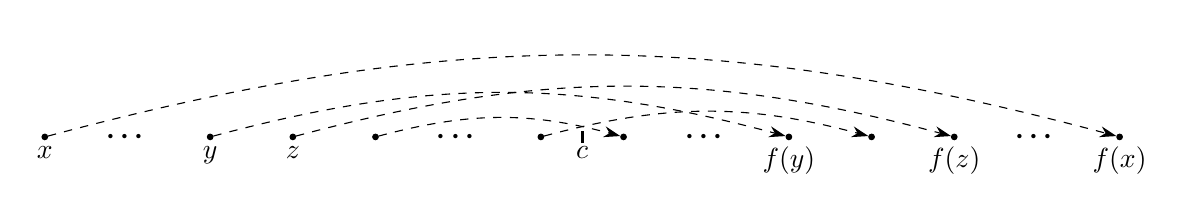
\begin{tikzpicture}

\tikzset{vertex/.style = {shape=circle, fill=black,draw,minimum size=2pt, inner sep=0pt}}
\tikzset{edge/.style = {->, >={Stealth[length=2.1mm, width=1.4mm]}}}
\tikzset{interval/.style = {<->,> = {Bracket[length=0.8mm, width=4mm]}, line width = 0.8pt}}

%help lines

% vertices
\node[vertex] (1) at  (0, 0) {};
\node (2) at (1.05, 0) {$\boldsymbol{\cdots}$};
\node[vertex] (3) at  (2.1, 0) {};
\node[vertex] (4) at  (3.15, 0) {};
\node[vertex] (5) at (4.2, 0) {};
\node (6) at (5.25, 0) {$\boldsymbol{\cdots}$};
\node[vertex] (7) at (6.3, 0) {};
\node (c) at (6.825, 0) {};
\draw[very thick] (6.825,-0.08) -- (6.825,0.08);
\node[vertex] (8) at (7.35, 0) {};
\node (9) at (8.4, 0) {$\boldsymbol{\cdots}$};
\node[vertex] (10) at  (9.45, 0) {};
\node[vertex] (11) at  (10.5, 0) {};
\node[vertex] (12) at (11.55, 0) {};
\node (13) at (12.6, 0) {$\boldsymbol{\cdots}$};
\node[vertex] (14) at  (13.65, 0) {};


\node[below] at (1) {$x$};
\node[below] at (c) {$c$};
\node[below] at (3) {$y$};
\node[below] at (4) {$z$};
\node[below] at (10) {$f(y)$};
\node[below] at (12) {$f(z)$};
\node[below] at (14) {$f(x)$};


%edges
\draw[edge, dashed] (1) to[bend left=15] (14);
\draw[edge, dashed] (3) to[bend left=15] (10);
\draw[edge, dashed] (4) to[bend left=15] (12);
\draw[edge, dashed] (5) to[bend left=15] (8);
\draw[edge, dashed] (7) to[bend left=15] (11);
%\draw[edge, white, line width = 2pt] (1) to[bend left=20] (4);
%\draw[edge, dashed] (1) to[bend left=20] (4);

%intervals

%oznake
%\Loop[dist=1cm,dir=NO,label=$$,labelstyle=above](1)  

%\draw[edge, dashed] (2)  to[bend right] (3);
%\draw[edge] (6) to[bend left] (4);

%\draw[edge] (1) to[bend left] (2);
%\draw[edge] (2) to[bend left] (1);

%\path (a2) to node {\dots} (c);
%\node [shape=circle,minimum size=1.5em] (a3) at (4.5,0) {};
%\draw[edge] (a2) to[bend left] (a3);
%\draw[edge] (a3) to[bend left] (a2);

%\node [shape=circle,minimum size=1.5em] (c1) at (6.5,0) {};
%\draw[edge] (c) to[bend left] (c1);
%\draw[edge] (c1) to[bend left] (c);
\end{tikzpicture}


\end{document} 